\chapter[Introdução]{Introdução}

Esse capítulo apresenta uma visão geral do trabalho através da definição do problema tratado, dos objetivos, 
da metodologia e dos resultados esperados.

\section{Problema}

O Sistema Integrado de Gestão Acadêmica(SiGA)\footnotemark é um sistema de controle acadêmico e financeiro de um Instituto de Educação.
\footnotetext{Repositório do SiGA - https://github.com/Sistema-Integrado-Gestao-Academica/SiGA} Este sistema é desenvolvido em PHP com a utilização do \textit{framework}
CodeIgniter. 
Durante o desenvolvimento, percebeu-se que o mesmo possui uma estrutura de testes muito precária, contando
apenas com uma classe de testes unitários com poucos recursos, sem a possibilidade de testes de integração. 

Na comunidade do PHP, um dos \textit{frameworks} de testes mais utilizados é o PHPUnit, que oferece diversos recursos para testes unitários e de integração.
Além disso, por ser um \textit{framework} de testes bastante utilizado pela comunidade, o PHPUnit é suportado na maioria de ferramentas
de integração contínua, o que favorece ainda mais a sua utilização. Todavia, o CodeIgniter não oferece suporte nativo ao PHPUnit
e existem algumas peculiaridades do CodeIgniter que devem ser levadas em conta, o que dificulta o uso do PHPUnit no CodeIgniter.

Essa deficiência em testes do \textit{framework} compromete a qualidade dos sistemas que o utilizam,
como o SiGA. Portanto, a questão de pesquisa que dirige este trabalho é:

\textit{Como adequar o PHPUnit para uso no CodeIgniter?}
  
\section{Objetivos}

  Nesta seção são apresentados os objetivos geral e específicos do trabalho definidos a fim de responder a
  questão de pesquisa definida.

\subsection{Objetivo Geral}

O objetivo geral deste trabalho é elaborar um \textit{framework} básico de testes para o CodeIgniter utilizando o PHPUnit, com suporte a 
testes unitários e de integração, para adequar o PHPUnit ao CodeIgniter.

\subsection{Objetivos Específicos}

São objetivos específicos deste trabalho:

\begin{itemize}
 \item Adaptar o CodeIgniter para utilizar o PHPUnit;
 \item Adequar o PHPUnit para uso no CodeIgniter;
 \item Levantar \textit{features} do \textit{framework} de testes, com base nas necessidades do CodeIgniter;
 \item Selecionar \textit{features} a serem implementadas;
 \item Implementar as \textit{features} selecionadas;
 \item Avaliar o \textit{framework} de testes criado, aplicando-o no SiGA.
\end{itemize}


\section{Metodologia}

  Como metodologia de execução do trabalho será realizada uma pesquisa-ação. De acordo com \citeonline{artigo_pesquisa_acao}, 
a pesquisa-ação pode ser caracterizada de várias formas. Para este trabalho será utilizada a pesquisa-ação iterativa e participatória.

Segundo \citeonline{artigo_pesquisa_acao}, a pesquisa-ação tem como objetivo entender uma situação em um contexto prático e melhorar esse contexto por meio de uma ação.
Dessa forma, essa metodologia foi escolhida dado o objetivo de construção de um \textit{framework} de testes para melhoria do \textit{framework} CodeIgniter.

A pesquisa-ação participatória ocorre quando o pesquisador tem uma participação ativa na implementação da ação e na produção das observações acerca do contexto estudado, também participa do compartilhamento de experiências da aplicação da ação. Uma pesquisa-ação iterativa consiste em uma ação dividida em ciclos. \cite{artigo_pesquisa_acao}

A ação a ser proposta é composta de um diagnóstico que é definido por \citeonline{artigo_pesquisa_acao} como uma fase que tem como objetivo principal conhecer a situação atual. Os ciclos de ação definidos para este trabalho tem como base as outras fases definidas por \citeonline{artigo_pesquisa_acao}: Planejamento da ação, Execução da ação e Avaliação da ação.

No diagnóstico serão estudados:
	\begin{itemize}
		\item O \textit{framework} de testes PHPUnit para entender as suas funcionalidades;
		\item O \textit{framework} CodeIgniter para entender como adequá-lo para uso do PHPUnit;
		\item Serão definidas todas as \textit{features} do \textit{framework} a ser criado.
	\end{itemize}

Para cada ciclo serão planejadas as atividades a serem realizadas para implementação do \textit{framework}.
Após o planejamento, essas atividades serão realizadas.
No final de cada ciclo será realizada uma avaliação do \textit{framework} por meio
de sua aplicação em um sistema (Sistema Integrado de Gestão Acadêmica - SiGA). A partir dessa aplicação serão identificadas
melhorias para as \textit{features} implementadas e até possíveis novas \textit{features}. 

A avaliação do \textit{framework} proposto e a identificação de melhorias serão realizadas por meio da avaliação qualitativa 
das respostas ao questionário (Apêndice \ref{questionario}) que será aplicado a dois desenvolvedores do sistema SiGA após utilizarem
o \textit{framework} para realizar determinados testes.


\section{Resultados Esperados}

Como resultado é esperado um \textit{framework} básico de testes para ser utilizado no \textit{framework} CodeIgniter, que contemple
testes unitários e testes de integração. Com a utilização da pesquisa-ação também é esperado que o \textit{framework} seja realmente adequado
ao CodeIgniter. Esse \textit{framework} será disponibilizado em um repositório público\footnote{https://github.com/VerVal-2016-1/Ignitest}.

\section{Cronograma}

A execução do trabalho foi organizada conforme Figura \ref{fig:cronograma}.

\begin{figure}[!htb]
\centering
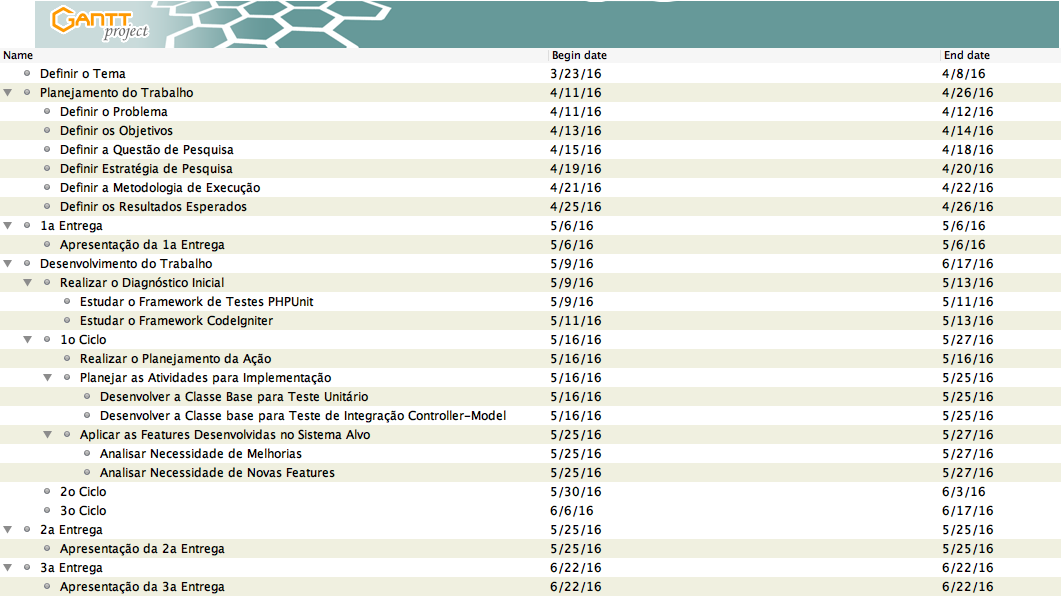
\includegraphics[scale=0.45]{figuras/Cronograma.png}
\caption{Cronograma}
\label{fig:cronograma}
\end{figure}
